\documentclass[../main.tex]{subfiles}
\begin{document}

\chapter{Головоломка MU}

\subsection{Формальные системы}

ОДНИМ ИЗ центральных понятий этой книги является понятие \emph{формальной системы}. Формальные системы того типа, который я использую, были изобретены американским логиком Эмилем Постом в 1920-х годах; их часто называют \emph{системами продукции} или \emph{системами Поста}. Эта глава познакомит вас с одной из таких формальных систем. Надеюсь, что вам захочется хотя бы немного её исследовать \--- чтобы вас заинтересовать, я придумал небольшую головоломку.

Головоломка формулируется просто: «Можете ли вы получить \textbf{MU}?»
Для начала вам будет дана некая строчка (последовательность букв).\footnote{Далее в книге, говоря о строчках, мы будем использовать следующие знаки: когда строчка будет напечатана тем же шрифтом, как и окружающий её текст, она будет заключена в простые или двойные кавычки. Знаки препинания, принадлежащие тексту, будут, как того требует логика, вне кавычек. Например, первая буква этой фразы \--- «Н», в то время, как первая буква «этой фразы» \--- «э». Однако, когда строчка будет напечатана другим шрифтом или латинским алфавитом, кавычки использоваться не будут \--- за исключением тех случаев, когда это будет абсолютно необходимо для ясности. Например, первая буква stola \--- s.}
Чтобы не мучить вас неизвестностью, сообщу эту строчку сразу \--- это будет MI.
Кроме этого, вам будут даны правила, с помощью которых вы сможете превращать одну строчку в другую.
Вы можете использовать любое правило, применимое в данный момент; при этом, если таких правил несколько, у вас имеется свободный выбор.
Именно в этот момент игра с формальной системой ближе всего подходит к искусству.
Само собой, главное требование игры \--- следование правилам.
Это ограничение может быть названо «требованием формальности».
Возможно, что в данной главе нам не придется подробно на нем останавливаться.
Однако, как бы удивительно это вам не казалось, работая с формальными системами последующих глав, вы увидите, что вам частенько захочется нарушать требование формальности, если у вас раньше не было навыка работы с подобными системами.

Наша формальная система \--- назовем её \emph{системой \textbf{MIU}} \--- использует лишь три буквы: \textbf{М}, \textbf{U}, \textbf{I}.
Это означает, что единственными строчками системы \textbf{MIU} будут те, которые используют только эти буквы.
Ниже приводятся некоторые строчки системы \textbf{MIU}:

\begin{itemize}[label={}, noitemsep, topsep=2pt, leftmargin=\parindent]
    \item \textbf{MU}
    \item \textbf{UIM}
    \item \textbf{MUUMUU}
    \item \textbf{UIIUMIUUIMUIIUMIUUIMUIIU}
\end{itemize}

Однако, хотя все эти строчки и правильны, вы ещё не можете ими распоряжаться.
Пока у вас имеется единственная строчка \--- \textbf{MI}.
Вы можете расширить вашу «коллекцию» путем применения правил.
Первое правило нашей системы:

\begin{mybox}{ПРАВИЛО I}
    Если у вас есть строчка, кончающаяся на \textbf{I}, вы можете прибавить \textbf{U} в конце.
\end{mybox}

Кстати, надо отметить, если вы уже сами об этом не догадались, что в понятии «строчка» важен определенный порядок букв. Например, \textbf{MI} и \textbf{IM} \--- две разные строчки. Строчка символов совсем не то же самое, что «мешок» с символами, где порядок символов не играет никакой роли.

Второе правило нашей системы:

\begin{mybox}{ПРАВИЛО II}
    Если у вас имеется \textbf{М}\textit{x}, вы можете прибавить к вашей коллекции \textbf{М}\textit{xx}.
\end{mybox}

Поясним это правило на нескольких примерах.

\begin{itemize}[label={}, noitemsep, topsep=6pt, leftmargin=\parindent]
    \item Из \textbf{MIU} вы можете получить \textbf{MIUIU}.
    \item Из \textbf{MUM} вы можете получить \textbf{MUMUM}.
    \item Из \textbf{MU} вы можете получить \textbf{MUU}.
\end{itemize}

Таким образом, буква~\textit{x} означает здесь любую строчку; однако, после того, как вы выбрали определенную строчку, вам придется держаться вашего выбора до тех пор, пока вы не используете снова то же правило \--- тогда вы можете сделать новый выбор.
Обратите внимание на третий пример. Он показывает, каким образом вы можете получить новую строчку из \textbf{MU} \--- но сначала вам необходимо иметь в вашей коллекции \textbf{MU}!
Хочу добавить ещё одно, последнее замечание, касающееся буквы «\textit{x} » она не является частью формальной системы в том смысле, как буквы «\textbf{М} », «\textbf{I} » и «\textbf{U} ». Тем не менее, нам нужен способ говорить о строчках системы вообще \--- и в этом нам помогает «\textit{x}», символизирующий любую произвольную строчку. Если в вашей коллекции оказывается строчка, содержащая «\textit{x}», это значит, что вы где-то ошиблись, так как в строчках системы \textbf{MIU} эта буква не встречается.

Третье правило нашей системы:

\begin{mybox}{ПРАВИЛО III}
    Если в какой-либо строчке встречается \textbf{III}, вы можете получить новую строчку, где вместо \textbf{III} будет \textbf{U}.
\end{mybox}

Примеры:

\begin{itemize}[label={}, noitemsep, topsep=6pt, leftmargin=\parindent]
    \item Из \textbf{UMIIIMU} вы можете получить \textbf{UMUMU}.
    \item Из \textbf{MIIII} вы можете получить \textbf{MIU} (а также \textbf{MUI}).
    \item Из \textbf{IIMII} вы не можете, применяя правило III, получить ничего нового. (Все три \textbf{I} должны стоять подряд.)
\end{itemize}

Ни в коем случае нельзя думать, что это правило можно применять в обратном порядке, как в следующем примере:

\begin{itemize}[label={}, noitemsep, topsep=6pt, leftmargin=\parindent]
    \item Из \textbf{MU} можно получить \textbf{MIII}. $\Leftarrow$ Это неверно.
\end{itemize}

Все правила читаются только в одном направлении, слева направо.

Последнее правило нашей системы:

\begin{mybox}{ПРАВИЛО IV}
    Если в какой-либо строчке встречается последовательность \textbf{UU}, вы можете её опустить.
\end{mybox}

\begin{itemize}[label={}, noitemsep, topsep=6pt, leftmargin=\parindent]
    \item Из \textbf{UUU} можно получить \textbf{U}.
    \item Из \textbf{MUUUIII} можно получить \textbf{MUIII}.
\end{itemize}

Теперь у вас есть все, что нужно, чтобы попытаться вывести \textbf{MU}.
Не волнуйтесь, если у вас не будет получаться; просто попробуйте поиграть с системой и постарайтесь схватить суть головоломки \textbf{MU}.
Надеюсь, что вы получите удовольствие!


\subsection{Теоремы, аксиомы и правила}

Ответ на головоломку \textbf{MU} вы найдете дальше в тексте.
Сейчас для нас важен сам процесс поиска решения.
Возможно, что вы уже попытались это сделать; если так, то теперь у вас оказалась целая коллекция строчек.
Подобные строчки, выведенные путем применения правил, называются \emph{теоремами}.
Термин «теорема», разумеется, широко используется в математике и имеет там совсем другое значение: какое-либо утверждение на естественном языке, доказанное с помощью строгих рассуждений (например, Теорема Зенона о «невозможности» движения или Теорема Эвклида о бесконечном количестве простых чисел).
Однако в формальных системах теоремы \--- не утверждения, а лишь строчки символов.
Такие теоремы не \emph{доказываются}, а просто \emph{производятся} автоматически при помощи неких типографских правил.
Чтобы подчеркнуть это важное отличие, в дальнейшем, говоря о «теоремах» в обыденном значении, я буду писать это слово с заглавной буквы: Теорема \--- это утверждение на каком-либо естественном языке, которое было доказано с помощью логических рассуждений.
Слово «теорема», написанное с маленькой буквы, будет употребляться в техническом значении: теорема \--- это строчка, выводимая в какой-либо формальной системе.
В этих терминах головоломка \textbf{MU} состоит в том, чтобы выяснить, является ли \textbf{MU} теоремой системы \textbf{MIU}.

В начале этой главы я «подарил» вам теорему \textbf{MI}.
Такая «дареная» теорема называется \emph{аксиомой}.
Также и в этом случае, техническое значение этого слова отличается от повседневного.
Формальная система может иметь ноль, одну, несколько и даже бесконечное множество аксиом.
Далее в книге приводятся примеры формальных систем всех трех видов.

Каждая формальная система обладает набором правил обращения с символами, таких, как четыре правила системы \textbf{MIU}.
Подобные правила называются \emph{порождающими правилами} или \emph{правилами вывода}; в дальнейшем я буду пользоваться обоими терминами.

И, наконец, последний термин \--- \emph{вывод}.
Ниже приводится вывод теоремы \textbf{MUIIU}:

\begin{block}
\begin{tabular}{@{} r @{~} l @{\quad} l @{}}
    (1) & \textbf{MI} & аксиома \\
    (2) & \textbf{MII} & из (1) по правилу II \\
    (3) & \textbf{MIIII} & из (2) по правилу II \\
    (4) & \textbf{MIIIIU} & из (3) по правилу I \\
    (5) & \textbf{MUIU} & из (4) по правилу III \\
    (6) & \textbf{MUIUUIU} & из (5) по правилу II \\
    (7) & \textbf{MUIIU} & из (6) по правилу IV \\
\end{tabular}
\end{block}

Выводом теоремы называется последовательное, шаг за шагом, объяснение того, как можно получить данную теорему согласно правилам формальной системы.
Понятие вывода основывается на понятии доказательства, являясь, однако, лишь его дальним родственником.
Было бы странным утверждать, что мы \emph{доказали} строчку \textbf{MUIIU}; скорее, мы её \emph{вывели}.


\subsection{Внутри и снаружи системы}

Большинство читателей, пытаясь решить головоломку \textbf{MU}, начинает выводить теоремы наобум и смотрят, что при этом получается. Вскоре, однако, они замечают, что полученные теоремы обладают некими свойствами; в этот момент в работу включается разум. Возможно, что пока вы не вывели несколько теорем, для вас не было очевидным, что все они будут начинаться с \textbf{M}. В какой-то момент вы заметили некую закономерность и смогли её объяснить, исходя из правил они таковы; что каждая новая теорема наследует первую букву предыдущей. В~результате первые буквы всех теорем восходят к первой букве нашей единственной аксиомы \textbf{MI} \--- и это доказательство того, что все теоремы системы \textbf{MIU} должны начинаться с~\textbf{M}.

То, что произошло, очень важно. Это указывает на одно из различий между человеком и машиной. Было бы возможно \--- и даже весьма нетрудно \--- запрограммировать компьютер на вывод теорем системы \textbf{MIU} ; мы можем включить в программу команду, велящую машине не останавливаться, пока она не выведет~\textbf{U}. Читатель уже знает, что компьютер, запрограммированный таким образом, не остановится никогда.

В этом нет ничего удивительного. Но что, если бы вы попросили вывести~\textbf{U} одного из ваших приятелей? Вы не удивились бы, если бы он через некоторое время подошел к вам, жалуясь, что он никак не может избавиться от~\textbf{M}, и что эти поиски \--- сумасбродная затея.

Даже не очень сообразительный человек не может не заметить закономерности в том, что он делает; эти наблюдения помогают ему лучше понять поставленную перед ним задачу. Компьютерная программа, которую мы только что упомянули, этого сделать не может.

Когда я сказал, что этот факт показывает различие между человеком и машиной, я имел в виду следующее: компьютер \emph{возможно} запрограммировать таким образом, что тот никогда не заметит даже самых очевидных закономерностей в том, что он делает; человеку, однако, свойственно подмечать определенные закономерности в его занятиях. Все это читатель, конечно, знал и раньше. Если вы возьмете калькулятор, нажмете на~1, прибавите~1, снова прибавите~1, и будете делать то же самое ещё много раз подряд, калькулятор никогда не научится делать этого сам; однако любой человек очень быстро заметил бы схему в ваших действиях Еще один простой пример: автомобиль, как бы долго и хорошо его не водили, никогда не научится избегать аварий и никогда не выучит даже самые частые маршруты своего хозяина.

Таким образом, различие в том, что машина \emph{может} не делать наблюдений, в то время как для человека это невозможно. Заметьте, что я не говорю, что \emph{вообще никакие} машины не способны делать сложных наблюдений; я имею в виду лишь некоторые из них. Я также не хочу сказать, что все люди способны делать сложные наблюдения; на самом деле, многие из них весьма ненаблюдательны. Но~машины, в отличие от людей, могут быть сделаны \emph{совершенно} ненаблюдательными. На самом деле, большинство машин, созданных до сих пор, весьма близки к полной ненаблюдательности; именно поэтому, многие считают, что отсутствие наблюдательности \--- одна из основных характеристик машин. Например, говоря о «механической» работе, мы не имеем в виду, что люди не могут с ней справиться; мы хотим сказать, что только машина способна безропотно проделывать такую работу снова и снова.


\subsection{Прыжки за пределы системы}

Человеческому интеллекту свойственно умение, выпрыгивая за пределы системы, смотреть на то, что он делает, со стороны; при этом он ищет \--- и часто находит \--- какую-либо схему, закономерность. В то же время, сказав, что разум способен взглянуть на свою работу со стороны, я не говорю, что он делает это всегда. Зачастую, однако, для этого бывает достаточно лишь небольшого толчка. Например, человеку, читающему книгу, может захотеться спать. Вместо того, чтобы дочитать книгу до конца, он, скорее всего, отложит её в сторону и потушит свет. При этом он «выходит из системы»; нам это кажется вполне естественным. Другой пример: человек А смотрит телевизор. В комнату входит человек Б и показывает явное неудовольствие ситуацией. Человек А может решить, что он понимает, в чем дело, и попытаться исправить положение, выходя из данной системы (той программы телевизора, которую он смотрел) и переключая телевизор на другой канал в поисках лучшей передачи. Б, однако, может иметь в виду более радикальный «выход из системы» \--- а именно, вообще выключить телевизор! В некоторых случаях только редкие личности могут заметить систему, управляющую жизнью многих людей \--- систему, никогда раньше таковой не считавшуюся. Подобные личности зачастую посвящают жизнь тому, чтобы убедить остальных, что система действительно существует, и что из нее необходимо выйти!

Насколько хорошо можно научить компьютер выскакивать за пределы системы? Я приведу пример, в свое время удививший многих наблюдателей. Не так давно на шахматном чемпионате среди компьютеров у одной из программ (самой слабой) оказалась необычайная особенность \--- сдаваться задолго до конца партии. Она не была хорошим игроком, зато умела увидеть, когда позиция становилась безнадежной, и сдаться в этот момент, вместо того, чтобы ждать, пока другая программа пройдет через скучную процедуру матования. Хотя та программа проиграла все свои партии, она сделала это с шиком, удивив многих местных знатоков шахмат. Таким образом, если мы определим здесь «систему» как «делать ходы шахматной партии», ясно, что та программа имела сложную, заранее запрограммированную способность выходить из системы. С другой стороны, если вы считаете, что «системой» в данном случае является «все то, что компьютер запрограммирован делать», несомненно, что та программа вовсе не умела выходить из системы.

Изучая формальные системы, очень важно отличать работу \emph{внутри} системы от наших наблюдений \emph{над} системой. Наверное, подобно большинству читателей, вы начали работу над головоломкой \textbf{MU} внутри системы; однако в какой-то момент ваше терпение истощилось и вы вышли из системы, пытаясь проанализировать результаты вашей работы и понять, почему вам до сих пор не удалось получить \textbf{MU}. Возможно, вы смогли ответить на этот вопрос; это \--- пример размышления о системе. Вероятно, в какой-то момент вы вывели \textbf{MIU} ; это \--- пример работы внутри системы. Я не хочу сказать, что эти два метода совершенно несовместимы; напротив, я уверен, что любой человек до определенной степени способен одновременно работать внутри системы и размышлять над тем, что он делает. Более того, в человеческих делах часто почти невозможно точно отделить работу внутри системы от её анализа; жизнь состоит из такого количества сложных, переплетенных между собой систем, что подобное деление вообще кажется слишком большим упрощением. Однако сейчас для нас важно четко сформулировать простые идеи, чтобы в дальнейшем мы могли опираться на них при анализе более сложных систем. Именно поэтому я рассказываю вам о формальных системах; кстати, нам пора вернуться к обсуждению системы \textbf{MIU}.


\subsection{Режим М, Режим I, Режим U.}

Головоломка \textbf{MU} была сформулирована таким образом, чтобы читатель некоторое время работал внутри системы, выводя теоремы. В то же время, её формулировка не обещала, что, оставаясь внутри системы, он сможет добиться результата. Таким образом, система \textbf{MIU} предполагает некоторое колебание между двумя режимами работы. Эти режимы можно разделить, используя два листа бумаги: на одном из них вы работаете «в качестве машины», заполняя лист теоремами; на другом вы работаете «в качестве мыслящего существа» и можете делать все, что вам подскажет смекалка: использовать русский язык, записывать идеи, работать в обратном порядке, использовать иксы, сжимать несколько шагов в один, менять правила системы, чтобы посмотреть, что из этого выйдет \--- короче, все, что придет вам в голову. Вы можете заметить, что числа 3 и 2 играют важную роль в системе, так как \textbf{I} сокращаются группами по 3, a \textbf{U} \--- группами по 2; кроме того, правило II позволяет удвоение букв (кроме \textbf{M} ). На втором листе бумаги у вас могут содержаться какие-то размышления по этому поводу. Позже мы ещё вернемся к этим двум способам работы с формальными системами; мы будем называть их механический режим (способ \textbf{M} ) и интеллектуальный режим (способ \textbf{I} ). Каждой букве системы \textbf{MIU} соответствует один из режимов. В дальнейшем я опишу последний режим \--- ультра-режим (режим \textbf{U} ), свойственный дзен-буддистскому подходу к вещам. Подробнее об этом через несколько глав.


\subsection{Алгоритм разрешения}

Работая над этой головоломкой, вы, вероятно, заметили, что она включает правила двух противоположных типов \emph{удлиняющие} и \emph{укорачивающие}. Два правила (I~и~II) позволяют нам удлинять строчки (естественно, лишь строго определенным образом), два других правила позволяют укорачивать строчки (опять же, следуя строгому закону). Кажется, что порядок применения этих правил можно бесконечно варьировать; таким образом, возникает надежда, что рано или поздно мы придем к искомой строчке~\textbf{MU}. Возможно, нам придется создать для этого гигантскую строчку и затем сокращать её, пока не останутся только два символа; или, того хуже, нам придется попеременно удлинять и сокращать, удлинять и сокращать, и так далее. При этом успех не гарантирован. На самом деле, мы уже заметили, что получить~\textbf{U} вообще невозможно, даже если бы мы удлиняли и сокращали строчки до второго пришествия.

Тем не менее, кажется, что с \textbf{MU} ситуация иная, чем с~\textbf{U}. Наше заключение о том, что \textbf{U} вывести невозможно, основывалось на очевидном свойстве этой строчки она не начинается с~\textbf{M}, как все остальные теоремы. Иметь такой простой способ отличать не-теоремы весьма удобно. Однако кто может поручиться, что подобный способ укажет нам \emph{все} не-теоремы? Вполне возможно, что существует множество начинающихся с~\textbf{M} строчек, которые, тем не менее, невыводимы. Это означало бы, что проверка «по первой букве» указывает нам только на ограниченное количество не-теорем, оставляя «за бортом» все остальные. Однако существует возможность найти некий более сложный метод проверки, точно говорящий нам, какие строчки могут быть выведены с помощью данных правил, а~какие \--- нет. Тут перед нами возникает вопрос: что мы подразумеваем под словом «проверка»? Читателю может быть не совсем понятно, какой смысл задаваться этим вопросом и почему он столь важен в данном контексте. Приведу пример такой «проверки», которая, как кажется, идет вразрез с самим смыслом этого слова.

Представьте себе джинна, в распоряжении которого имеется все время на свете. Джинн тратит это время на вывод теорем системы \textbf{MIU}. Делает он это весьма методично, скажем, следующим образом:

\begin{itemize}[
    noitemsep,
    topsep=4pt,
    label={},
    leftmargin=\parindent,
]
    \item Шаг 1: Приложить все подходящие правила к аксиоме \textbf{MI}. \\
    Это дает две новые теоремы: \textbf{MIU}, \textbf{MII}.

    \item Шаг 2: Приложить все подходящие правила к теоремам, полученным в шаге~1. \\
    Это дает три новые теоремы: \textbf{MIIU}, \textbf{MIUIU}, \textbf{MIIII}.

    \item Шаг 3: Приложить все подходящие правила к теоремам, полученным в шаге~2. \\
    Это дает пять новых теорем: \textbf{MIIIIU}, \textbf{MIIUIIU}, \textbf{MIUIUIUIU}, \textbf{МIIIIIIII}, \textbf{MUI}.

    \item \quad$\bm{\vdots}$
\end{itemize}

Следуя этому методу, рано или поздно мы выведем каждую теорему системы, так как правила применяются во всех мыслимых комбинациях. (См.~рис.~\ref{fig:miu-tree})
Все удлиняющие и укорачивающие трансформации, упомянутые выше, со временем будут осуществлены.

\begin{figure}
    \centering
    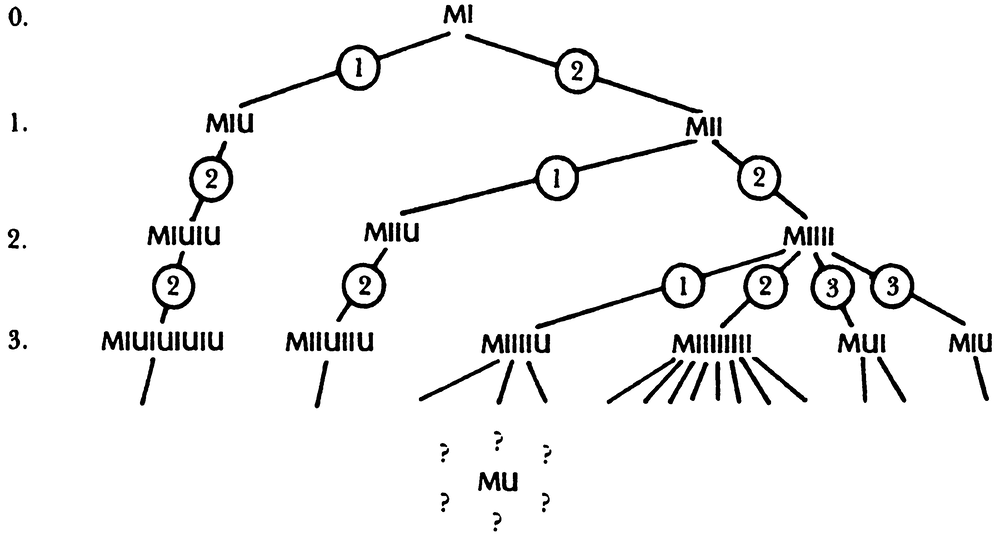
\includegraphics[width=0.9\textwidth]{img/miu-tree.png}
    \caption{Систематически построенное «дерево» всех теорем системы~\textbf{MIU}. {$N$-ный} уровень внизу содержит теоремы, для вывода которых понадобилось ровно~$N$ шагов. Номера в кружках говорят нам, с помощью какого правила была получена данная теорема. Растет ли на этом дереве~\textbf{MU}?}
    \label{fig:miu-tree}
\end{figure}

Неясно, однако, как долго нам придется ждать появления той или иной строчки, поскольку теоремы расположены согласно длине их вывода. Это не очень-то полезное расположение, в особенности, если вы заинтересованы в какой-то определенной строчке (например,~\textbf{MU}) и при этом не знаете не только того, какой длины её вывод, но даже того, существует ли этот вывод вообще. Теперь давайте взглянем на обещанную «проверку теоремности»:

Ждите, пока данная строчка будет выведена; когда это случится, вы будете знать, что это \--- теорема. Если же этого не случится никогда, вы можете быть уверены, что данная строчка \--- не теорема.

Это звучит нелепо, так как здесь имеется в виду, что мы согласны ждать ответа до скончания веков. Таким образом, мы опять подошли к вопросу о том, что может считаться «проверкой». Прежде всего, нам необходима гарантия, что мы получим ответ за ограниченный промежуток времени. Такая проверка теоремности, которая завершается в конечный отрезок времени, называется \emph{алгоритмом разрешения} для данной формальной системы.

Когда у вас имеется алгоритм разрешения, все теоремы системы приобретают конкретную характеристику. С первого взгляда может показаться, что правила и аксиомы формальной системы сами по себе характеризуют её теоремы не менее полно, чем алгоритм разрешения; однако проблема здесь заключается в слове «характеризуют». Безусловно, как правила вывода, так и аксиомы системы \textbf{MIU} косвенно характеризуют строчки, являющиеся теоремами; ещё более косвенно они характеризуют строчки, теоремами \emph{не}~являющиеся. Однако косвенная характеристика часто недостаточна. Если кто-нибудь утверждает, что он имеет в своем распоряжении характеристику всех теорем, но при этом тратит бесконечное время, чтобы установить, что данная строчка не является теоремой, вы, скорее всего, подумаете, что в его характеристике чего-то не хватает \--- она недостаточно конкретна. Именно поэтому так важно установить, есть ли в данной системе алгоритм разрешения. Положительный ответ будет означать, что вы всегда можете проверить, является ли данная строчка теоремой; при этом, какой бы длинной проверка ни была, она \emph{непременно придет к концу}. В принципе, проверка \--- такой же простой, механический, конечный и верный процесс, как установление того, что первая буква строчки \--- \textbf{M}. Алгоритм разрешения \--- это «лакмусовая бумажка» для установления теоремности!

Кстати, одним из требований формальной системы является наличие алгоритма разрешения для аксиом: каждая формальная система должна иметь свою Лакмусовую бумажку для определения аксиомности. Таким образом, у нас не будет проблем по крайней мере в начале работы. Разница между множеством аксиом и множеством теорем в том, что первые всегда имеют алгоритм разрешения, в то время как последние могут его и не иметь.

Уверен, что вы согласитесь, что, когда вы начали работать с системой \textbf{MIU}, вам пришлось столкнуться именно с этой проблемой. Вам была известна единственная аксиома системы и простые правила вывода, косвенно характеризующие теоремы \--- и все же было неясно, каковы последствия этой характеристики. В частности, было совершенно непонятно, является ли \textbf{MU} теоремой.

\begin{figure}
    \centering
    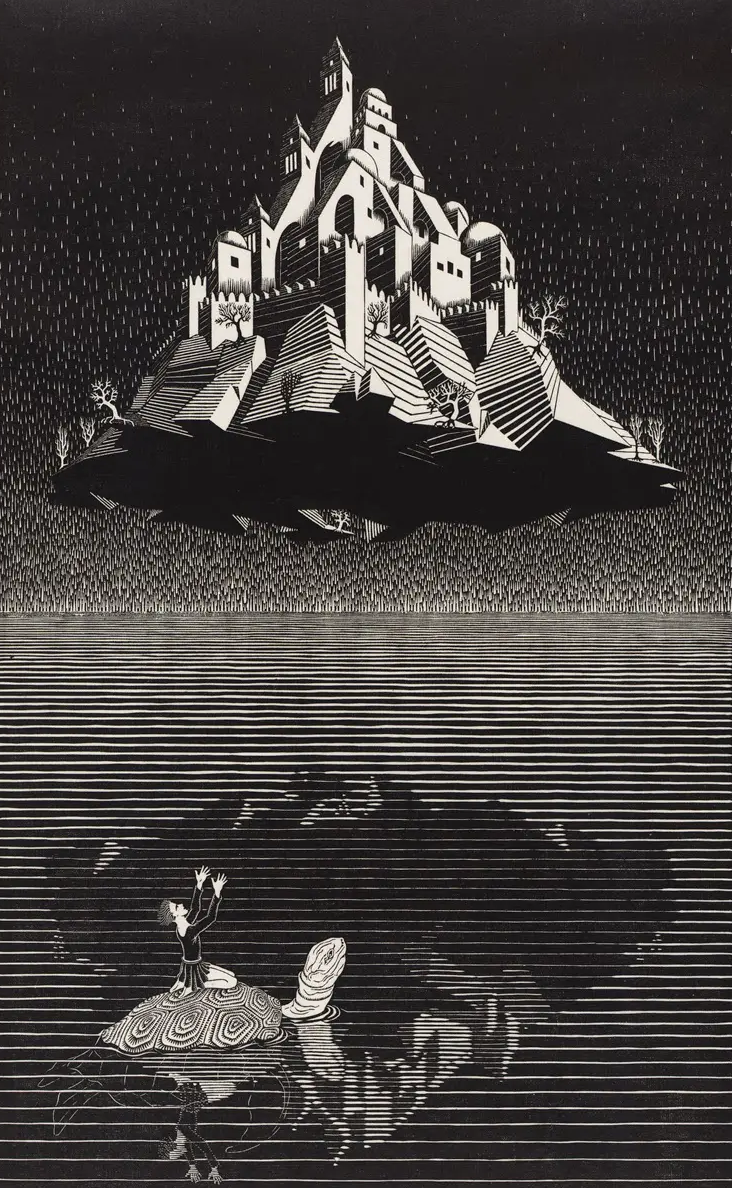
\includegraphics[max width=\textwidth, max totalheight=\textheight-2\baselineskip]{img/escher-castle-in-the-air.png}
    \caption{М.К.~Эшер. «Воздушный замок» (гравюра на дереве), 1928}
    \label{fig:escher-castle}
\end{figure}

\end{document}
